\section{Results}\label{sec:results}

Our goal was to evaluate our agents in specific scenarios, and to compare different kinds of agents to each other. To this end, we introduced parametricity in their emotional reactions. While the interplay of affect, decision-making and belief generation was the same in all agents, as was the schema of their emotional reactions, the strength of these reactions varied --- while all agents feared dying, for instance, not all feared it to the same degree. Similarly, while all felt fear in the proximity of a Wumpus, they felt it with different intensities.

We parametrised our agents through five criteria, with two possible values for each. These were:

\begin{itemize}
	\item anger, with the possible values \emph{strong}/\emph{weak};
	\item fear, with the possible values \emph{strong}/\emph{weak};
	\item enthusiasm, with the possible values \emph{strong}/\emph{weak};
	\item contentment, with the possible values \emph{strong}/\emph{weak};
	\item hostility, with the values \emph{hostile}/\emph{friendly}.
\end{itemize}

Note that each emotion of the PSBC is represented by one criterion, while the emotions of the SJS were rolled into one for the sake of simplicity. For each emotion or \emph{personality fragment}, we constructed a graph consisting of approximately $10^4$ nodes by hand\footnote{Of course, we generated large parts of these graphs through templating as well, as there had many repeating structures.}, with output nodes that had configurable significances. These graphs are far too large for explication here\footnote{The code of the implementation is accessible at \url{https://github.com/jtapolczai/wumpus}.} and there was, indeed, no special theory behind their construction, but we did use common-sense assumptions which we will illustrate by listing a few output nodes:

\begin{itemize}
	\item High health reduced fear.
	\item The presence of a Wumpus with low health increased anger. Closer Wumpuses generated more anger than distant ones.
	\item Dying significantly increased fear.\footnote{While such a node might seem useless, agents can receive ``You have died''-messages from their belief generators.}
	\item Items lying on the ground increased enthusiasm.
	\item Low health also increased enthusiasm, so as to induce the enthusiasm-related action of eating,
	\item Empty cells increased contentment.
	\item Eating fruit or meat decreased enthusiasm as a way of signalling satisfaction.
	\item Killing a Wumpus decreased anger.
\end{itemize}

Each output node had a variable significance which we varied according to whether we wanted the emotion to be strong or weak or hostile or friendly, respectively. The concrete values for these significances were, again, the product of intuition. For an agent with strong fear, dying increased the value by 0.8 out of a possible 1, making it almost certain that a ``You have died''-message would lead fear to override all other emotions. For weak fear, the value only increased by 0.5 --- still very high, but considerably lower, and possible to override if the agent's anger was strong enough. The five criteria induced 32 possibly combinations of values, with each combination representing a possible personality for an agent.

For convenience, we will use the shorthand notation of Definition~\ref{def:personality} to specify an agent's personality.

\begin{definition}\label{def:personality}
   Let $A$ be an agent and let $P_A = \tuple{\field{X}_a, \field{X}_f, \field{X}_e, \field{X}_c, \field{X}_h}$ with $\field{X}_a, \field{X}_f, \field{X}_e, \field{X}_c \in \{ \type{W}, \type{S} \}$ and $\field{X}_h \in \{ \type{H}, \type{F} \}$.
   
   Then $P_A$ is a specification for a $A$'s personality, with $\field{X}_a$, $\field{X}_f$, $\field{X}_e$, $\field{X}_c$, $\field{X}_h$ representing the agent's personality fragments for anger, fear, enthusiasm, and hostility, respectively. The values $\type{W}$ and $\type{S}$ stand for a \emph{weak} or \emph{strong} fragment, while $\type{H}$ and $\type{F}$ will stand for a \emph{hostile} or \emph{friendly} value for hostility.
\end{definition}

\subsection{Qualitative Evaluation}

To evaluate the general fitness of our architecture, we placed one or two agents in a number of scenarios with a clear expected outcome. Unless otherwise noted, we expected all personalities to perform in the same way.

\paragraph{Scenario: harvesting a single plant.} The first scenario was a 5x5 world with two ripe plants and an agent with a health of 0.6 that had food in its inventory. The agent's health was low, but eating one plant would restore it to a level of 1.1. We expected the agent to move to the closest plant, harvest it, eat the fruit now it its inventory, and then rest. We can see the world in Figure~\ref{fig:evalWorld1} and the actions of the agent in Listing~\ref{lst:evalWorld1}. Coordinates are given in the format $(x,y)$.

\begin{figure}[h]
	\centering
		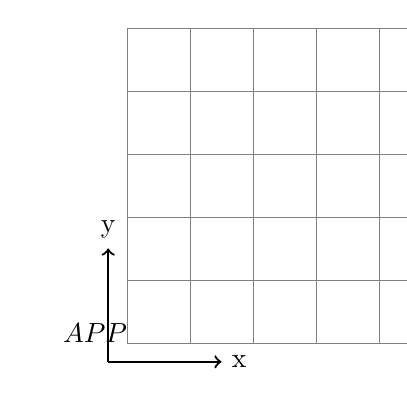
\begin{tikzpicture}[scale=0.8]	
		\figBlueCube{(2,1)}{$\fontsize{9.5pt}{1em}A$}
		\figDarkGreenCube{(2,2)}{$\fontsize{9.5pt}{1em}P$}
		\figDarkGreenCube{(2,4)}{$\fontsize{9.5pt}{1em}P$}
		
		\draw[thick,->] (-0.3,-0.3) -- (1.5,-0.3) node[anchor=west] {x};
		\draw[thick,->] (-0.3,-0.3) -- (-0.3,1.5) node[anchor=south] {y};

		\draw[step=1cm,gray,very thin] (0,0) grid (5,5);
	\end{tikzpicture}
	\caption{The world of the scenario ``harvesting a single plant''. In the South, we have a single agent labelled $A$. The green squares labelled $P$ indicate plants.}
	\label{fig:evalWorld1}
\end{figure}

\begin{lstlisting}[caption=Actions in the scenario ``harvesting a single plant''., label=lst:evalWorld1]
A at (2,0) moved North to (2,1).
A at (2,1) harvested a plant.
A at (2,1) ate Fruit.
A at (2,1) did nothing.
A at (2,1) did nothing.
\end{lstlisting}

As we can see, the agent performed according to our expectations.

\paragraph{Scenario: harvesting all plants.} This scenario was identical to the previous one, save for the agent's health, which was set at 0.1. Very close to dying, we expected the agent to harvest both plants and eat both fruits in succession to increase its health above 1. We see the actions of the agent in in Listing~\ref{lst:evalWorld2}. The agent again performed according to our expectations.

\noindent
\begin{minipage}{\linewidth}
\begin{lstlisting}[caption=Actions in the scenario ``harvesting all plants''., label=lst:evalWorld2]
A at (2,0) moved North to (2,1).
A at (2,1) harvested a plant.
A at (2,1) ate Fruit.
A at (2,1) moved North to (2,2).
A at (2,2) moved North to (2,3).
A at (2,3) harvested a plant.
A at (2,3) ate Fruit.
A at (2,3) did nothing.
A at (2,3) did nothing.
\end{lstlisting}
\end{minipage}

\paragraph{Scenario: resting.} This scenario is the simplest: we place an agent in good health into an empty 5x5 world. We expect it to simply stay put for a short while, avoiding exertion, or to look around to ascertain its surroundings. Listing~\ref{lst:evalWorld3} shows the results. Since we had not built in any notion of curiosity into our agents, they simply remained in place, which we deemed acceptable behaviour.

\begin{lstlisting}[caption=Actions in the scenario ``resting''., label=lst:evalWorld3]
A at (2,2) did nothing.
A at (2,2) did nothing.
A at (2,2) did nothing.
A at (2,2) did nothing.
A at (2,2) did nothing.
\end{lstlisting}

\paragraph{Scenario: killing a wounded Wumpus.} Here we put a Wumpus with 0.1 health at some distance from a healthy agent, with the expectation that any agent would attack such a weak enemy, regardless of personality. The world is shown in Figure~\ref{fig:evalWorld4} and the agent's actions are shown in Listing~\ref{lst:evalWorld4}. We can see that the agent indeed approached and killed the wounded Wumpus. However, Enthusiasm then replaced anger as its dominant emotion and the agent collected the meat from the corpse. This was both surprising and beneficial behaviour, as there was nothing else do and an agent can always use additional food in its inventory.

\begin{figure}
	\centering
		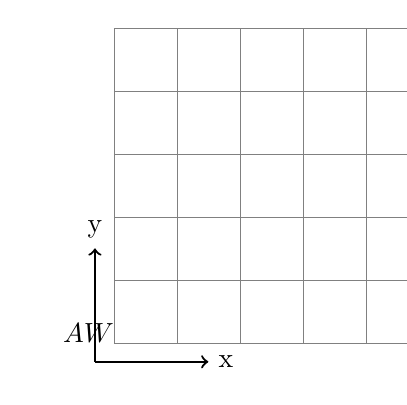
\begin{tikzpicture}[scale=0.8]	
		\figBlueCube{(2,1)}{$\fontsize{9.5pt}{1em}A$}
		\figRedCube{(2,4)}{$\fontsize{9.5pt}{1em}W$}
		
		\draw[thick,->] (-0.3,-0.3) -- (1.5,-0.3) node[anchor=west] {x};
		\draw[thick,->] (-0.3,-0.3) -- (-0.3,1.5) node[anchor=south] {y};

		\draw[step=1cm,gray,very thin] (0,0) grid (5,5);
	\end{tikzpicture}
	\caption{The world of the scenario ``killing a wounded Wumpus''. In the South, we have a single agent labelled $A$. To its north, we have wounded Wumpus labelled $W$.}
	\label{fig:evalWorld4}
\end{figure}

\noindent
\begin{minipage}{\linewidth}
\begin{lstlisting}[caption=Actions in the scenario ``killing a wounded Wumpus''., label=lst:evalWorld4]
W at (2,3) moved South to (2,2).
A at (2,0) moved North to (2,1).
A at (2,1) attacked w1 to its North.
A at (2,1) moved North to (2,2).
A at (2,2) picked up Meat.
A at (2,2) ate Meat.
A at (2,2) did nothing.
A at (2,2) did nothing.
\end{lstlisting}
\end{minipage}

\paragraph{Scenario: picking up items.} An agent with low health was placed into a world in which two cells had items: one had 2 pieces of meat and another, most distant one, had 3 pieces of fruit. We expected the agent to collect the items and eat as many as necessary to restore its health to at least 1. Figure~\ref{fig:evalWorld5} shows the world and Listing~\ref{lst:evalWorld5} the results. We can see that the agent was killed in both cases, though for different reasons: in the first, the agent killed the closer Wumpus, but this reduced its health to 0.4. When the second Wumpus came close, the agent began moving backwards until it reached the edge of the world, whereupon the Wumpus killed it. In the second case, the agent was controlled by anger, not by fear. It had picked up the meat from the first Wumpus as the second approached it but, instead of eating, the agent immediately and suicidally attacked the Wumpus. In both cases, the agent's behaviour was suboptimal, as it could have eaten the meat from the first Wumpus and thereby regain enough health to survive the second's attack --- however, if we conceive of the first agent running away in fear and the second attacking in blind anger, we can at least make intuitive sense of their actions.

\begin{figure}
	\centering
		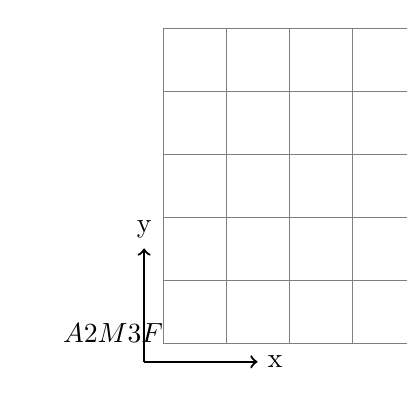
\begin{tikzpicture}[scale=0.8]	
		\figBlueCube{(2,1)}{$\fontsize{9.5pt}{1em}A$}
		\figLightRedCube{(2,3)}{$\fontsize{9.5pt}{1em}2M$}
		\figLightGreenCube{(3,3)}{$\fontsize{9.5pt}{1em}3F$}
		
		\draw[thick,->] (-0.3,-0.3) -- (1.5,-0.3) node[anchor=west] {x};
		\draw[thick,->] (-0.3,-0.3) -- (-0.3,1.5) node[anchor=south] {y};

		\draw[step=1cm,gray,very thin] (0,0) grid (5,5);
	\end{tikzpicture}
	\caption{The world of the scenario ``picking up items''. In the South, we have a single agent labelled $A$. To its north we have a cell with 2 pieces of meat, labelled $2M$, and another cell with 3 pieces of fruit, labelled $3F$.}
	\label{fig:evalWorld5}
\end{figure}

\begin{lstlisting}[caption=Actions in the scenario ``picking up items''., label=lst:evalWorld5]
A at (2,0) moved North to (2,1).
A at (2,1) moved North to (2,2).
A at (2,2) picked up Meat.
A at (2,2) ate Meat.
A at (2,2) ate Meat.
A at (2,2) did nothing.
A at (2,2) did nothing.
\end{lstlisting}

\paragraph{Scenario: fight or flight.}  Similarly to the scenario ``killing a wounded Wumpus'', we placed an agent together with two Wumpuses, each with a health of 0.6. An agent was able to win the fight against both by first killing one, eating its meat to restore its health, and then killing the second. In this scenario, we wanted to test the interplay between anger and fear --- accordingly, we expected agents with different personalities to react in different ways. Figure~\ref{evalWorld6} shows the world; Listing~\ref{lst:evalWorld6_1} shows the actions of an agent with the personality $\personality{W}{W}{W}{W}{F}$, Listing~\ref{lst:evalWorld6_2} the actions of an agent with the personality $\personality{S}{W}{S}{W}{F}$. Our expectation was that the first agent would try to take fly in the face of danger, whereas the second would try to fight, perhaps suicidally so.

\begin{figure}
    \centering
    	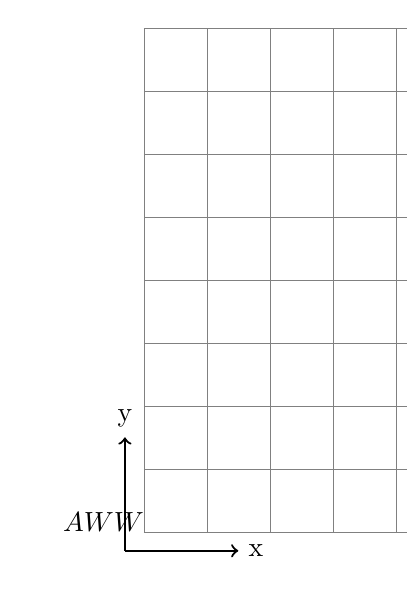
\begin{tikzpicture}[scale=0.8]	
		\figBlueCube{(2,2)}{$\fontsize{9.5pt}{1em}A$}
        \figRedCube{(2,4)}{$\fontsize{9.5pt}{1em}W$}
        \figRedCube{(2,8)}{$\fontsize{9.5pt}{1em}W$}
		
		\draw[thick,->] (-0.3,-0.3) -- (1.5,-0.3) node[anchor=west] {x};
		\draw[thick,->] (-0.3,-0.3) -- (-0.3,1.5) node[anchor=south] {y};

		\draw[step=1cm,gray,very thin] (0,0) grid (5,8);
	\end{tikzpicture}
    \caption{The world of the scenario ``fight or flight''. We have an agent labelled $A$ and two Wumpuses labelled $W1$ and $W2$.}
    \label{fig:evalWorld6}
\end{figure}

\begin{lstlisting}[caption=Actions of an agent with the personality $\personality{W}{W}{W}{W}{F}$ in the scenario ``fight or flight''., label=lst:evalWorld6_1]
   A at (2,0) moved North to (2,1).
   W1 at (2,3) moved South to (2,2).
   W2 at (2,7) moved South to (2,6).
   A at (2,1) attacked W1 to its North.
   W2 at (2,6) moved South to (2,5).
   A at (2,1) moved North to (2,2).
   W2 at (2,5) moved South to (2,4).
   A at (2,2) moved South to (2,1).
   W2 at (2,4) moved South to (2,3).
   A at (2,1) moved South to (2,0).
   W2 at (2,3) moved South to (2,2).
   A at (2,0) did nothing.
   W2 at (2,2) moved South to (2,1).
   A at (2,0) did nothing.
   W2 at (2,1) attacked A to its South.
\end{lstlisting}

\begin{lstlisting}[caption=Actions of an agent with the personality $\personality{S}{W}{S}{W}{F}$ in the scenario ``fight or flight''., label=lst:evalWorld6_2]
   A at (2,0) moved North to (2,1).
   W1 at (2,3) moved South to (2,2).
   W2 at (2,7) moved South to (2,6).
   A at (2,1) attacked W2 to its North.
   W2 at (2,6) moved South to (2,5).
   A at (2,1) moved North to (2,2).
   W2 at (2,5) moved South to (2,4).
   A at (2,2) picked up Meat.
   W2 at (2,4) moved South to (2,3).
   A at (2,2) attacked W2 to its North.
\end{lstlisting}

\paragraph{Scenario: searching for food.} We placed an agent with 0.5 health into a world with one pile of fruit outside of its sight cone. This scenario was interesting because, while the goal was clear, there was no obvious series of actions which the agent was supposed to take, nor was a goal immediately obvious. We expected it to search its surroundings in search of a source of food. The world is shown in Figure~\ref{fig:evalWorld7} and the results in Listing~\ref{lst:evalWorld7}. It should be noted that the agent's actions are largely random, as agents may randomly select a possible action if several equally beneficial are possible. As we can see, the results were somewhat unsatisfying. While the agent did eventually find the food, it spent many round aimlessly wandering and turning around. Due to the lack of any dedicated algorithm responsible for exploration and the lack of stimuli to guide it, the agent essentially moved around randomly until it eventually stumbled upon the cell with meat on it.

\begin{figure}
    \centering
    	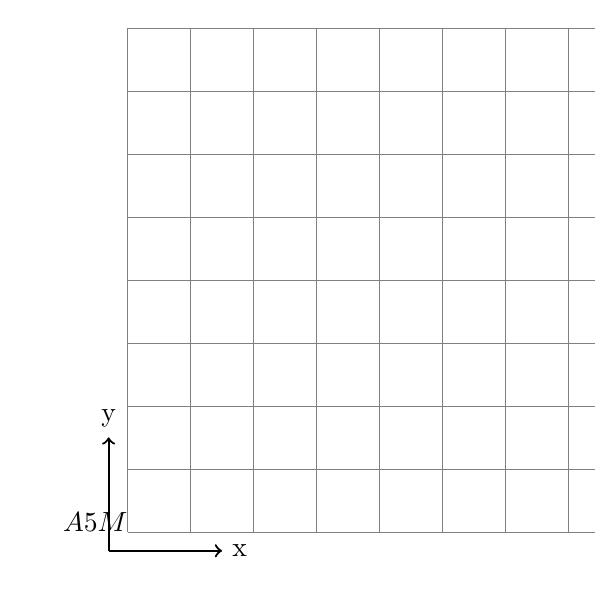
\begin{tikzpicture}[scale=0.8]	
		\figBlueCube{(3,1)}{$\fontsize{9.5pt}{1em}A$}
        \figLightRedCube{(3,8)}{$\fontsize{9.5pt}{1em}5M$}
		
		\draw[thick,->] (-0.3,-0.3) -- (1.5,-0.3) node[anchor=west] {x};
		\draw[thick,->] (-0.3,-0.3) -- (-0.3,1.5) node[anchor=south] {y};

		\draw[step=1cm,gray,very thin] (0,0) grid (8,8);
	\end{tikzpicture}
    \caption{The world of the scenario ``searching for food''. We have an agent labelled $A$ and a cell with 5 pieces of meat labelled $5M$.}
    \label{fig:evalWorld7}
\end{figure}

\begin{lstlisting}[caption=Actions in the scenario ``searching for food''., label=lst:evalWorld7]
A at (3,0) moved North to (3,1).
A at (3,1) turned West.
A at (3,1) moved West to (2,1).
A at (2,1) moved West to (1,1).
A at (1,1) moved West to (0,1).
A at (0,1) turned South.
A at (0,1) turned North.
A at (0,1) turned South.
A at (0,1) turned North.
A at (0,1) turned South.
A at (0,1) turned North.
A at (0,1) moved East to (1,1).
A at (1,1) moved East to (2,1).
A at (2,1) moved North to (2,2).
A at (2,2) moved North to (2,3).
A at (2,3) moved North to (2,4).
A at (2,4) moved North to (2,5).
A at (2,5) moved East to (3,5).
A at (3,5) moved North to (3,6).
A at (3,6) moved North to (3,7).
A at (3,7) picked up Meat.
A at (3,7) ate Meat.
A at (3,7) did nothing.
\end{lstlisting}

\paragraph{Scenario: giving a gift to a friend.} Here we placed two agents, first with the personalities $\personality{W}{W}{W}{W}{F}$ and then $\personality{W}{W}{S}{W}{F}$ in a 5x5 world and added fruit to the inventory of $A$. Though their disposition towards each other was neutral, we expected them to interact in a friendly way, by giving items and sending sympathy-related gestures. Figure~\ref{fig:evalWorld8} shows the world and Listing~\ref{lst:evalWorld8_1} shows somewhat interesting the results. In the case of weak enthusiasm, instead of approaching $B$, $A$ just ate the food and then remained in place, content. $B$, on the other hand, approached $A$ and started sending the gesture \emph{love}, which we hard-coded as the friendly one. $A$'s contentment overwhelmed its enthusiasm once its health was sufficiently high. Though this behaviour was unexpected and we could have changed it by adjusting emotional filters, we did deem $A$ selfishness in its interaction with what was essentially a stranger efficient. In the second case, in which both agents had strong enthusiasm, $A$ was more charitable. As we seen in Listing~\ref{lst:evalWorld8_2}, $A$ chose to share after eating one item of meat.

\begin{figure}
    \centering
    	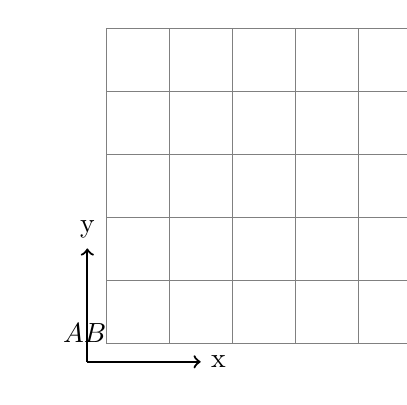
\begin{tikzpicture}[scale=0.8]	
		\figBlueCube{(2,1)}{$\fontsize{9.5pt}{1em}A$}
        \figBlueCube{(2,5)}{$\fontsize{9.5pt}{1em}B$}
		
		\draw[thick,->] (-0.3,-0.3) -- (1.5,-0.3) node[anchor=west] {x};
		\draw[thick,->] (-0.3,-0.3) -- (-0.3,1.5) node[anchor=south] {y};

		\draw[step=1cm,gray,very thin] (0,0) grid (5,5);
	\end{tikzpicture}
    \caption{The world of the scenario ``giving a gift to a friend''. We have two agents labelled $A$ and $B$. $A$ has three pieces of fruit in its inventory.}
    \label{fig:evalWorld8}
\end{figure}

\begin{lstlisting}[caption=Actions in the scenario ``giving a gift to a friend'' when both agents had the personality $\personality{W}{W}{W}{W}{F}$., label=lst:evalWorld8_1]
A at (2,0) ate Fruit.
B at (2,4) moved South to (2,3).
A at (2,0) did nothing.
B at (2,3) moved South to (2,2).
A at (2,0) did nothing.
B at (2,2) moved South to (2,1).
A at (2,0) did nothing.
B at (2,1) gestured 'love' to A to its South.
A at (2,0) did nothing.
B at (2,1) gestured 'love' to A to its South.
\end{lstlisting}

\begin{lstlisting}[caption=Actions in the scenario ``giving a gift to a friend'' when both agents had the personality $\personality{W}{W}{S}{W}{F}$., label=list:evalWorld8_2]
A at (2,0) moved North to (2,1).
B at (2,4) moved South to (2,3).
A at (2,1) moved North to (2,2).
B at (2,3) gestured 'love' to 1 to its South.
A at (2,2) gave Meat to 2 to its North.
B at (2,3) gestured 'love' to 1 to its South.
A at (2,2) gestured 'love' to 2 to its North.
B at (2,3) gave Meat to 1 to its South.
A at (2,2) gestured 'love' to 2 to its North.
B at (2,3) gestured 'love' to 1 to its South.
\end{lstlisting}

\subsubsection{Results}

Our agents performed the basic tasks set to them reasonably well. Agents managed to acquire food if they knew the location of a food source, kill enemies if it seemed easy to do so, and have positive interactions with friendly agents. As we saw in the scenario ``fight or flight'', their personalities were also able to meaningfully influence their behaviour. Somewhat disappointing was the performance in ``searching for food'', where it became clear that the agents would have benefited from a drive to systematically explore their surroundings.

\subsection{Quantitative Evaluation}

For the second part of our evaluation, we placed 224 agents --- 7 of each of the 32 possible personalities in a hand-crafted, somewhat irregularly shaped, 100x100 world that contained some small forests of plants, seen in Figure~\ref{fig:evalWorldQuant}. We then distributed the agents, as well as $\left\lfloor 224/3 \right\rfloor = 74$ Wumpuses uniformly and randomly over all cells. We also placed additional plants and gold uniformly and randomly in the world such that, for all cells $(x,y)$ in the world,

$$
	\begin{array}{l l l}
		P(\textrm{A plant is added to cell } (x,y)) & = & 0.05\\
		P(\textrm{1 gold is added to cell } (x,y)) & = & 0.01\\
		P(\textrm{A pit is added to cell } (x,y)) & = & 0.01
	\end{array}
$$

We simulated the world for 200 rounds or until at least half of the agents died -- whichever came sooner. During the simulation, we recorded the survival rate of each of the 32 populations and that of the Wumpuses. The results are listed in Table~\ref{tab:evalSurvival} and shown graphically in Figure~\ref{fig:evalSurvival}.

\begin{figure}
	\centering
	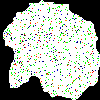
\includegraphics[width=400pt]{Figs/evalWorldQuant.png}
	\caption{The world of the quantitative evaluation, consisting of 100x100 cells. White pixels represent accessible cells, black pixels represent inaccessible ones. Green pixels represent plants, ochre ones pits, red ones Wumpuses and blue ones agents, where the value of the blue channel is the agent's ID. Orange pixels represent gold. The world's island shape was created by hand, while all entities and items were distributed randomly.}
	\label{fig:evalWorldQuant}
\end{figure}

\subsubsection{Results}

We ran the trial with each personality and captured the following data as we did so: the number of

\begin{itemize}
	\item harvests,
	\item attacks,
	\item gifts given (split by gift type),
	\item gestures sent,
	\item items eaten,
	\item surviving Wumpuses,
	\item surviving agents.
\end{itemize}

In addition to recording the raw numbers, we also calculated their averages by personality fragment to see whether there was a clear relation between certain personality types and success.

\paragraph{Number of harvests.} We see the number of harvests by personality type in Table~\ref{tab:numHarvests}, which shows a rather large difference between the personalities. Table~\ref{tab:numHarvestsAvg} shows the average number of harvests by personality fragment. As expected, strong enthusiasm and weak contentment led to the largest increase in harvest frequency, with fear, anger and hostility having negligible effects.

\paragraph{Number of attacks.} Table~\ref{tab:numAttacks} shows the number of attacks and Table~\ref{tab:numAttacksAvg} the averages. All personality fragments seemed to play a role in the agents' aggression: anger predictably increased it and fear lowered it, but strong enthusiasm and contentment lowered the number as well. Surprisingly, hostile agents actually performed slightly less attacks, which might be explained with the fact that they spent more time sending hostile gestures than friendly, as we shall see below.

\begin{table}
	\centering
	\makebox[0pt][c]{\parbox{\textwidth}{%
			\begin{minipage}[b]{0.42\hsize}\centering
				\begin{tabular}{ l | c }
					\emph{Personality} & \emph{Harvests} \\
					\hline
					$\personality{S}{W}{W}{S}{F}$ & 8\\
					$\personality{S}{W}{S}{S}{H}$ & 9\\
					$\personality{S}{W}{W}{S}{H}$ & 9\\
					$\personality{S}{W}{W}{W}{H}$ & 11\\
					$\personality{S}{S}{W}{S}{H}$ & 11\\
					$\personality{S}{W}{S}{S}{F}$ & 11\\
					$\personality{W}{W}{S}{S}{F}$ & 11\\
					$\personality{W}{W}{W}{S}{H}$ & 11\\
					$\personality{S}{S}{W}{S}{F}$ & 12\\
					$\personality{W}{W}{S}{S}{H}$ & 12\\
					$\personality{S}{S}{S}{S}{H}$ & 13\\
					$\personality{S}{S}{W}{W}{F}$ & 13\\
					$\personality{W}{S}{S}{S}{H}$ & 13\\
					$\personality{W}{W}{W}{W}{H}$ & 13\\
					$\personality{S}{S}{W}{W}{H}$ & 14\\
					$\personality{S}{W}{W}{W}{F}$ & 14\\
					$\personality{W}{W}{W}{S}{F}$ & 14\\
					$\personality{W}{W}{W}{W}{F}$ & 14\\
					$\personality{S}{S}{S}{S}{F}$ & 15\\
					$\personality{W}{S}{W}{S}{F}$ & 15\\
					$\personality{W}{S}{W}{S}{H}$ & 15\\
					$\personality{W}{S}{W}{W}{F}$ & 15\\
					$\personality{W}{S}{W}{W}{H}$ & 15\\
					$\personality{W}{S}{S}{S}{F}$ & 16\\
					$\personality{W}{W}{S}{W}{F}$ & 17\\
					$\personality{S}{W}{S}{W}{H}$ & 18\\
					$\personality{W}{S}{S}{W}{F}$ & 18\\
					$\personality{S}{W}{S}{W}{F}$ & 19\\
					$\personality{W}{W}{S}{W}{H}$ & 19\\
					$\personality{S}{S}{S}{W}{H}$ & 20\\
					$\personality{S}{S}{S}{W}{F}$ & 21\\
					$\personality{W}{S}{S}{W}{H}$ & 24\\
				\end{tabular}
				\caption{Number of plant harvests after 50 rounds.}
				\label{tab:numHarvests}
			\end{minipage}
			\hfill
			\begin{minipage}[b]{0.42\hsize}\centering
				\begin{tabular}{ l | c }
					\emph{Personality} & \emph{Attacks} \\
					\hline
						$\personality{S}{S}{S}{W}{H}$ & 1\\
						$\personality{W}{S}{S}{W}{H}$ & 2\\
						$\personality{W}{W}{S}{S}{F}$ & 2\\
						$\personality{W}{W}{S}{S}{H}$ & 2\\
						$\personality{S}{S}{S}{S}{F}$ & 3\\
						$\personality{W}{S}{S}{S}{H}$ & 3\\
						$\personality{W}{S}{W}{S}{F}$ & 3\\
						$\personality{W}{S}{W}{S}{H}$ & 3\\
						$\personality{S}{S}{S}{S}{H}$ & 4\\
						$\personality{S}{S}{W}{S}{H}$ & 4\\
						$\personality{W}{S}{S}{S}{F}$ & 4\\
						$\personality{W}{S}{W}{W}{F}$ & 4\\
						$\personality{S}{S}{S}{W}{F}$ & 5\\
						$\personality{W}{S}{W}{W}{H}$ & 5\\
						$\personality{W}{W}{W}{S}{F}$ & 5\\
						$\personality{W}{W}{W}{S}{H}$ & 5\\
						$\personality{S}{S}{W}{W}{H}$ & 6\\
						$\personality{S}{W}{S}{S}{H}$ & 6\\
						$\personality{S}{W}{S}{W}{H}$ & 6\\
						$\personality{W}{S}{S}{W}{F}$ & 6\\
						$\personality{W}{W}{S}{W}{H}$ & 6\\
						$\personality{W}{W}{W}{W}{F}$ & 6\\
						$\personality{W}{W}{W}{W}{H}$ & 6\\
						$\personality{S}{S}{W}{S}{F}$ & 7\\
						$\personality{S}{W}{S}{S}{F}$ & 8\\
						$\personality{S}{W}{S}{W}{F}$ & 8\\
						$\personality{S}{W}{W}{S}{F}$ & 8\\
						$\personality{S}{S}{W}{W}{F}$ & 9\\
						$\personality{W}{W}{S}{W}{F}$ & 9\\
						$\personality{S}{W}{W}{S}{H}$ & 10\\
						$\personality{S}{W}{W}{W}{F}$ & 11\\
						$\personality{S}{W}{W}{W}{H}$ & 12\\
				\end{tabular}
				\caption{Number of attacks after 50 rounds.}
				\label{tab:numAttacks}
			\end{minipage}
			\hfill
		}}
\end{table}

\begin{table}
	\centering
	\begin{tabular}{ l | c | c }
		\emph{Personality fragment} & \emph{weak/hostile} & \emph{ strong/friendly} \\
		\hline
		Anger & 15.125 & 13.625\\
		Fear & 13.125 & 15.625 \\
		Enthusiasm & 12.75 & 16 \\
		Contentment & 16.563 & 12.18 \\
		Hostility & 14.188 & 14.563 \\
		\hline
	\end{tabular}
	\caption{Average number of plant harvests, by personality fragment.}
	\label{tab:numHarvestsAvg}
\end{table}

\begin{table}
	\centering
	\begin{tabular}{ l | c | c }
		\emph{Personality fragment} & \emph{weak/hostile} & \emph{friendly/strong} \\
		\hline
		Anger & 4.438 & 6.75 \\
		Fear & 6.875 & 4.313 \\
		Enthusiasm & 6.5 & 4.688 \\
		Contentment & 6.375 & 4.813 \\
		Hostility & 5.063 & 6.125 \\
		\hline
	\end{tabular}
	\caption{Average number of attacks, by personality fragment.}
	\label{tab:numAttacksAvg}
\end{table}

\paragraph{Gifts given.} Tables~\ref{tab:numFruitGiven}-\ref{tab:numGoldGiven} show the number of gifts given and Tables~\ref{tab:numFruitGivenAvg}-\ref{tab:numGoldGivenAvg} show the averages. Immediately, we can see that meat was the most popular gift, followed by gold and fruit, which almost no agents gave. Most interesting is the case of meat: we see quite starkly that strong anger, weak fear, high enthusiasm and low contentment resulted in a population of apex predators that spent much of their time killing Wumpuses (and each other) and built up inventories that they shared with the survivors. Gold, too, is of note: as its acquisition did not require killing, high contentment and friendliness significantly increased the chance that it would be given as a gift. The unpopularity of fruit as gift is somewhat contrary to our expectations and shows that agents did not guard plants are reliably sources of food and did not infer that they would regularly regrow.

\begin{table}
	\centering
	\makebox[0pt][c]{\parbox{\textwidth}{%
			\begin{minipage}[b]{0.30\hsize}\centering
				\begin{tabular}{ l | c }
					\emph{Personality} & \emph{Gifts (fruit)} \\
					\hline
					$\personality{S}{W}{W}{W}{H}$ & 0\\
					$\personality{S}{S}{S}{S}{F}$ & 0\\
					$\personality{S}{S}{S}{S}{H}$ & 0\\
					$\personality{S}{S}{S}{W}{F}$ & 0\\
					$\personality{S}{S}{W}{S}{F}$ & 0\\
					$\personality{S}{S}{W}{S}{H}$ & 0\\
					$\personality{S}{S}{W}{W}{F}$ & 0\\
					$\personality{S}{S}{W}{W}{H}$ & 0\\
					$\personality{S}{W}{S}{S}{F}$ & 0\\
					$\personality{S}{W}{S}{S}{H}$ & 0\\
					$\personality{S}{W}{S}{W}{F}$ & 0\\
					$\personality{S}{W}{S}{W}{H}$ & 0\\
					$\personality{S}{W}{W}{S}{F}$ & 0\\
					$\personality{S}{W}{W}{S}{H}$ & 0\\
					$\personality{S}{W}{W}{W}{F}$ & 0\\
					$\personality{W}{S}{S}{S}{H}$ & 0\\
					$\personality{W}{S}{S}{W}{F}$ & 0\\
					$\personality{W}{S}{W}{S}{F}$ & 0\\
					$\personality{W}{S}{W}{S}{H}$ & 0\\
					$\personality{W}{S}{W}{W}{F}$ & 0\\
					$\personality{W}{W}{S}{S}{F}$ & 0\\
					$\personality{W}{W}{S}{S}{H}$ & 0\\
					$\personality{W}{W}{S}{W}{F}$ & 0\\
					$\personality{W}{W}{S}{W}{H}$ & 0\\
					$\personality{W}{W}{W}{S}{F}$ & 0\\
					$\personality{W}{W}{W}{S}{H}$ & 0\\
					$\personality{W}{W}{W}{W}{F}$ & 0\\
					$\personality{W}{W}{W}{W}{H}$ & 0\\
					$\personality{S}{S}{S}{W}{H}$ & 1\\
					$\personality{W}{S}{S}{W}{H}$ & 1\\
					$\personality{W}{S}{W}{W}{H}$ & 1\\
					$\personality{W}{S}{S}{S}{F}$ & 3\\
					\hline
				\end{tabular}
				\caption{Number of fruit items given as gifts after 50 rounds.}
				\label{tab:numFruitGiven}
			\end{minipage}
			\hfill
			\begin{minipage}[b]{0.30\hsize}\centering
				\begin{tabular}{ l | c }
					\emph{Personality} & \emph{Gifts (meat)} \\
					\hline
					$\personality{S}{W}{W}{W}{H}$ & 0\\
					$\personality{S}{S}{S}{S}{F}$ & 0\\
					$\personality{S}{S}{S}{S}{H}$ & 0\\
					$\personality{S}{S}{S}{W}{H}$ & 0\\
					$\personality{S}{S}{W}{S}{F}$ & 0\\
					$\personality{S}{S}{W}{S}{H}$ & 0\\
					$\personality{S}{S}{W}{W}{F}$ & 0\\
					$\personality{S}{S}{W}{W}{H}$ & 0\\
					$\personality{S}{W}{S}{S}{F}$ & 0\\
					$\personality{S}{W}{S}{S}{H}$ & 0\\
					$\personality{S}{W}{W}{S}{H}$ & 0\\
					$\personality{W}{S}{S}{S}{F}$ & 0\\
					$\personality{W}{S}{S}{S}{H}$ & 0\\
					$\personality{W}{S}{S}{W}{F}$ & 0\\
					$\personality{W}{S}{W}{S}{F}$ & 0\\
					$\personality{W}{S}{W}{S}{H}$ & 0\\
					$\personality{W}{S}{W}{W}{F}$ & 0\\
					$\personality{W}{W}{S}{S}{H}$ & 0\\
					$\personality{W}{W}{W}{S}{F}$ & 0\\
					$\personality{W}{W}{W}{W}{F}$ & 0\\
					$\personality{W}{W}{W}{W}{H}$ & 0\\
					$\personality{S}{W}{W}{S}{F}$ & 1\\
					$\personality{S}{W}{W}{W}{F}$ & 2\\
					$\personality{W}{S}{W}{W}{H}$ & 2\\
					$\personality{W}{W}{W}{S}{H}$ & 2\\
					$\personality{W}{W}{S}{W}{F}$ & 5\\
					$\personality{W}{W}{S}{S}{F}$ & 7\\
					$\personality{S}{S}{S}{W}{F}$ & 11\\
					$\personality{W}{W}{S}{W}{H}$ & 12\\
					$\personality{W}{S}{S}{W}{H}$ & 17\\
					$\personality{S}{W}{S}{W}{F}$ & 19\\
					$\personality{S}{W}{S}{W}{H}$ & 19\\
					\hline
				\end{tabular}
				\caption{Number of meat items given as gifts after 50 rounds.}
				\label{tab:numMeatGiven}
			\end{minipage}
			\hfill
			\begin{minipage}[b]{0.30\hsize}\centering
				\begin{tabular}{ l | c }
					\emph{Personality} & \emph{Gifts (gold)} \\
					\hline
					$\personality{S}{S}{S}{S}{F}$ & 0\\
					$\personality{S}{S}{S}{S}{H}$ & 0\\
					$\personality{S}{S}{W}{S}{F}$ & 0\\
					$\personality{S}{S}{W}{S}{H}$ & 0\\
					$\personality{S}{W}{S}{S}{F}$ & 0\\
					$\personality{S}{W}{S}{S}{H}$ & 0\\
					$\personality{S}{W}{S}{W}{H}$ & 0\\
					$\personality{S}{W}{W}{S}{F}$ & 0\\
					$\personality{S}{W}{W}{S}{H}$ & 0\\
					$\personality{W}{S}{S}{S}{F}$ & 0\\
					$\personality{W}{S}{S}{S}{H}$ & 0\\
					$\personality{W}{S}{S}{W}{F}$ & 0\\
					$\personality{W}{S}{S}{W}{H}$ & 0\\
					$\personality{W}{S}{W}{S}{F}$ & 0\\
					$\personality{W}{S}{W}{S}{H}$ & 0\\
					$\personality{W}{W}{S}{W}{F}$ & 0\\
					$\personality{W}{W}{S}{W}{H}$ & 0\\
					$\personality{W}{W}{W}{S}{F}$ & 0\\
					$\personality{W}{W}{W}{S}{H}$ & 0\\
					$\personality{S}{W}{W}{W}{H}$ & 1\\
					$\personality{S}{S}{W}{W}{F}$ & 1\\
					$\personality{S}{W}{W}{W}{F}$ & 1\\
					$\personality{W}{S}{W}{W}{F}$ & 1\\
					$\personality{W}{S}{W}{W}{H}$ & 1\\
					$\personality{W}{W}{S}{S}{H}$ & 1\\
					$\personality{W}{W}{W}{W}{H}$ & 1\\
					$\personality{S}{S}{S}{W}{F}$ & 2\\
					$\personality{S}{S}{W}{W}{H}$ & 2\\
					$\personality{W}{W}{S}{S}{F}$ & 2\\
					$\personality{W}{W}{W}{W}{F}$ & 2\\
					$\personality{S}{S}{S}{W}{H}$ & 5\\
					$\personality{S}{W}{S}{W}{F}$ & 6\\
					\hline
				\end{tabular}
				\caption{Number of gold items given as gifts after 50 rounds.}
				\label{tab:numGoldGiven}
			\end{minipage}
			\hfill
		}}
\end{table}


\begin{table}
	\centering
	\begin{tabular}{ l | c | c }
		\emph{Personality fragment} & \emph{weak/hostile} & \emph{ strong/friendly} \\
		\hline
		Anger & 0.313 & 0.063\\
		Fear & 0.0 & 0.375\\
		Enthusiasm & 0.063 & 0.313\\
		Contentment & 0.188 & 0.188\\
		Hostility & 0.188 & 0.188\\
		\hline
	\end{tabular}
	\caption{Average number of fruit gifts given, by personality fragment.}
	\label{tab:numFruitGivenAvg}
\end{table}

\begin{table}
	\centering
	\begin{tabular}{ l | c | c }
		\emph{Personality fragment} & \emph{weak/hostile} & \emph{friendly/strong} \\
		\hline
			Anger & 2.8125 & 3.25\\
			Fear & 4.1875 & 1.875\\
			Enthusiasm & 0.4375 & 5.625\\
			Contentment & 5.4375 & 0.625\\
			Hostility & 3.25 & 2.8125\\
		\hline
	\end{tabular}
	\caption{Average number of meat gifts given, by personality fragment.}
	\label{tab:numMeatGivenAvg}
\end{table}

\begin{table}
	\centering
	\begin{tabular}{ l | c | c }
		\emph{Personality fragment} & \emph{weak/hostile} & \emph{friendly/strong} \\
		\hline
		Anger & 0.5 & 1.125\\
		Fear & 0.875 & 0.75\\
		Enthusiasm & 0.625 & 1.0\\
		Contentment & 1.438 & 0.188\\
		Hostility & 0.688 & 0.938\\
		\hline
	\end{tabular}
	\caption{Average number of gold items given, by personality fragment.}
	\label{tab:numGoldGivenAvg}
\end{table}

\paragraph{Gestures.} Table~\ref{tab:numGestures} shows the number of gestures sent, Table~\ref{tab:numGesturesAvg} the averages. We can clearly see the dominant role of strong enthusiasm, followed distantly by weak contentment. This is very much according to our expectations, as gestures are primarily enthusiasm-associated. Anger, fear, and hostility only had relatively minor effects on the number of social interactions.
	
\paragraph{Items eaten.} We see the results and the averages in Table~\ref{tab:numMeals} and Table~\ref{tab:numMealsAvg}, respectively. Clearly, the two most significant factors here are strong enthusiasm and weak contentment. As eating is enthusiasm-related, it makes sense that agents with strong enthusiasm would eat more, as would agents with weak contentment, since food has to be acquired through action.
	
\begin{table}
	\centering
	\makebox[0pt][c]{\parbox{\textwidth}{%
			\begin{minipage}[b]{0.42\hsize}\centering
				\begin{tabular}{ l | c }
					\emph{Personality} & \emph{Gestures} \\
					\hline
						$\personality{W}{W}{W}{S}{H}$ & 30\\
						$\personality{S}{W}{W}{S}{H}$ & 32\\
						$\personality{S}{W}{W}{S}{F}$ & 34\\
						$\personality{W}{W}{W}{S}{F}$ & 40\\
						$\personality{W}{S}{W}{S}{H}$ & 46\\
						$\personality{S}{S}{W}{S}{H}$ & 61\\
						$\personality{W}{S}{W}{S}{F}$ & 66\\
						$\personality{S}{S}{W}{S}{F}$ & 69\\
						$\personality{S}{W}{W}{W}{F}$ & 92\\
						$\personality{S}{W}{W}{W}{H}$ & 116\\
						$\personality{S}{S}{W}{W}{F}$ & 120\\
						$\personality{W}{S}{W}{W}{F}$ & 124\\
						$\personality{W}{S}{W}{W}{H}$ & 129\\
						$\personality{W}{W}{W}{W}{F}$ & 129\\
						$\personality{W}{W}{W}{W}{H}$ & 132\\
						$\personality{S}{S}{W}{W}{H}$ & 136\\
						$\personality{S}{W}{S}{W}{F}$ & 309\\
						$\personality{S}{S}{S}{S}{H}$ & 335\\
						$\personality{W}{S}{S}{W}{F}$ & 359\\
						$\personality{W}{S}{S}{W}{H}$ & 361\\
						$\personality{W}{W}{S}{W}{F}$ & 373\\
						$\personality{S}{S}{S}{S}{F}$ & 388\\
						$\personality{S}{W}{S}{S}{F}$ & 394\\
						$\personality{S}{W}{S}{S}{H}$ & 397\\
						$\personality{W}{S}{S}{S}{F}$ & 403\\
						$\personality{S}{S}{S}{W}{F}$ & 405\\
						$\personality{S}{S}{S}{W}{H}$ & 411\\
						$\personality{W}{W}{S}{W}{H}$ & 439\\
						$\personality{S}{W}{S}{W}{H}$ & 451\\
						$\personality{W}{W}{S}{S}{H}$ & 452\\
						$\personality{W}{S}{S}{S}{H}$ & 494\\
						$\personality{W}{W}{S}{S}{F}$ & 495\\
						\hline
				\end{tabular}
				\caption{Number of gestures sent after 50 rounds.}
				\label{tab:numGestures}
			\end{minipage}
			\hfill
			\begin{minipage}[b]{0.42\hsize}\centering
				\begin{tabular}{ l | c }
					\emph{Personality} & \emph{Meals} \\
					\hline
						$\personality{S}{W}{S}{S}{H}$ & 10\\
						$\personality{S}{W}{S}{S}{F}$ & 11\\
						$\personality{S}{W}{W}{S}{F}$ & 11\\
						$\personality{S}{W}{W}{S}{H}$ & 11\\
						$\personality{S}{S}{W}{S}{H}$ & 12\\
						$\personality{W}{W}{S}{S}{F}$ & 12\\
						$\personality{W}{W}{S}{S}{H}$ & 12\\
						$\personality{W}{W}{W}{S}{H}$ & 12\\
						$\personality{S}{W}{W}{W}{H}$ & 13\\
						$\personality{S}{S}{S}{S}{H}$ & 13\\
						$\personality{S}{S}{W}{S}{F}$ & 13\\
						$\personality{W}{S}{S}{S}{H}$ & 13\\
						$\personality{S}{S}{W}{W}{H}$ & 14\\
						$\personality{W}{S}{W}{S}{H}$ & 14\\
						$\personality{W}{S}{W}{W}{H}$ & 14\\
						$\personality{W}{W}{W}{W}{H}$ & 14\\
						$\personality{S}{S}{S}{S}{F}$ & 15\\
						$\personality{S}{S}{W}{W}{F}$ & 15\\
						$\personality{W}{S}{W}{S}{F}$ & 15\\
						$\personality{W}{S}{W}{W}{F}$ & 15\\
						$\personality{W}{W}{W}{S}{F}$ & 15\\
						$\personality{W}{W}{W}{W}{F}$ & 15\\
						$\personality{W}{S}{S}{S}{F}$ & 16\\
						$\personality{S}{W}{S}{W}{F}$ & 18\\
						$\personality{S}{W}{W}{W}{F}$ & 18\\
						$\personality{S}{S}{S}{W}{H}$ & 19\\
						$\personality{W}{S}{S}{W}{F}$ & 19\\
						$\personality{S}{S}{S}{W}{F}$ & 20\\
						$\personality{S}{W}{S}{W}{H}$ & 20\\
						$\personality{W}{W}{S}{W}{F}$ & 20\\
						$\personality{W}{W}{S}{W}{H}$ & 20\\
						$\personality{W}{S}{S}{W}{H}$ & 24\\
						\hline
				\end{tabular}
				\caption{Number of items eaten after 50 rounds.}
				\label{tab:numMeals}
			\end{minipage}
			\hfill
		}}
\end{table}

\begin{table}
	\centering
	\begin{tabular}{ l | c | c }
		\emph{Personality fragment} & \emph{weak/hostile} & \emph{ strong/friendly} \\
		\hline
			Anger & 254.5 & 234.375\\
			Fear & 244.688 & 244.188\\
			Enthusiasm & 84.75 & 404.125\\
			Contentment & 255.375 & 233.5\\
			Hostility & 251.375 & 237.5\\
		\hline
	\end{tabular}
	\caption{Average number of gestures sent, by personality fragment.}
	\label{tab:numGesturesAvg}
\end{table}

\begin{table}
	\centering
	\begin{tabular}{ l | c | c }
		\emph{Personality fragment} & \emph{weak/hostile} & \emph{friendly/strong} \\
		\hline
			Anger & 15.625 & 14.563\\
			Fear & 14.5 & 15.688\\
			Enthusiasm & 13.813 & 16.38\\
			Contentment & 17.375 & 12.813\\
			Hostility & 14.688 & 15.5\\
		\hline
	\end{tabular}
	\caption{Average number items eaten, by personality fragment.}
	\label{tab:numMealsAvg}
\end{table}

\paragraph{Surviving Wumpuses.} We see the absolute number of surviving Wumpuses and the averages in Table~\ref{tab:numWumpuses} and Table~\ref{tab:numWumpusesAvg}. Similarly to the number of meat gifts given, we see that strong anger, weak fear and low contentment all led to more Wumpuses being killed. Enthusiasm and hostility somewhat increased the Wumpuses' chances of survival --- here we might hypothesize that agents with strong enthusiasm spent more time gathering fruit and engaging in interactions with other agents, and that hostile agents spent more time attacking each other than they spent attacking Wumpuses.

\paragraph{Surviving agents.} The absolute and average number of surviving agents are listed in Table~\ref{tab:numAgents} and Table~\ref{tab:numAgents}. While all other metrics were important as well, in the end, survival by whatever means is the measure of success in our evaluation. While all personality types managed to survive reasonable well, we can see significant differences between them. In Table~\ref{tab:numAgentsAvg}, we can see that agents with weak anger survived better than those with strong anger, as did agents with strong fear. This does make sense, as fighting was a dangerous tactic, despite the meat with which it provided the victor. High enthusiasm had a moderately beneficial effect on survival, which again makes since, as it is associated with low-cost, high-reward behaviour like the gathering of food and items and the sending of friendly gestures that might lead to gifts in the future. Contentment had relatively little effect and hostility actually increased survival. The case of hostility is somewhat odd, as we would have expected friendliness to have the same beneficial effect that enthusiasm in general had, but it seems that not being too friendly by perhaps giving away all of one's inventory to others might also be advantageous.

\begin{table}
	\centering
	\makebox[0pt][c]{\parbox{\textwidth}{%
			\begin{minipage}[b]{0.42\hsize}\centering
				\begin{tabular}{ l | c }
					\emph{Personality} & \emph{Agents} \\
					\hline
					$\personality{S}{W}{W}{W}{H}$ & 20\\
					$\personality{S}{W}{W}{S}{H}$ & 20\\
					$\personality{S}{S}{W}{W}{F}$ & 21\\
					$\personality{S}{W}{S}{S}{H}$ & 21\\
					$\personality{S}{W}{S}{W}{F}$ & 21\\
					$\personality{S}{W}{W}{S}{F}$ & 21\\
					$\personality{W}{S}{S}{W}{F}$ & 21\\
					$\personality{W}{W}{S}{W}{F}$ & 21\\
					$\personality{S}{S}{S}{S}{H}$ & 22\\
					$\personality{S}{S}{W}{S}{F}$ & 22\\
					$\personality{S}{S}{W}{W}{H}$ & 22\\
					$\personality{S}{W}{S}{S}{F}$ & 22\\
					$\personality{S}{W}{W}{W}{F}$ & 22\\
					$\personality{W}{W}{W}{S}{H}$ & 22\\
					$\personality{W}{W}{W}{W}{H}$ & 22\\
					$\personality{W}{W}{W}{S}{F}$ & 23\\
					$\personality{W}{W}{W}{W}{F}$ & 23\\
					$\personality{S}{S}{S}{S}{F}$ & 24\\
					$\personality{S}{S}{S}{W}{F}$ & 24\\
					$\personality{S}{S}{W}{S}{H}$ & 24\\
					$\personality{W}{S}{W}{W}{H}$ & 24\\
					$\personality{S}{W}{S}{W}{H}$ & 25\\
					$\personality{W}{S}{W}{W}{F}$ & 25\\
					$\personality{W}{W}{S}{S}{F}$ & 25\\
					$\personality{W}{W}{S}{S}{H}$ & 25\\
					$\personality{S}{S}{S}{W}{H}$ & 26\\
					$\personality{W}{S}{S}{S}{F}$ & 26\\
					$\personality{W}{S}{S}{S}{H}$ & 26\\
					$\personality{W}{S}{S}{W}{H}$ & 26\\
					$\personality{W}{S}{W}{S}{F}$ & 26\\
					$\personality{W}{W}{S}{W}{H}$ & 26\\
					$\personality{W}{S}{W}{S}{H}$ & 27\\
					\hline
				\end{tabular}
				\caption{Number of surviving agents after 50 rounds.}
				\label{tab:numAgents}
			\end{minipage}
			\hfill
			\begin{minipage}[b]{0.42\hsize}\centering
				\begin{tabular}{ l | c }
					\emph{Personality} & \emph{Wumpuses} \\
					\hline
					$\personality{S}{S}{W}{W}{F}$ & 3\\
					$\personality{S}{W}{W}{W}{F}$ & 3\\
					$\personality{S}{W}{W}{W}{H}$ & 4\\
					$\personality{S}{W}{S}{W}{H}$ & 4\\
					$\personality{W}{W}{S}{W}{F}$ & 4\\
					$\personality{S}{W}{W}{S}{H}$ & 5\\
					$\personality{W}{S}{W}{W}{H}$ & 5\\
					$\personality{S}{S}{S}{W}{F}$ & 6\\
					$\personality{S}{S}{S}{W}{H}$ & 6\\
					$\personality{S}{S}{W}{S}{F}$ & 6\\
					$\personality{S}{W}{S}{S}{F}$ & 6\\
					$\personality{S}{W}{S}{S}{H}$ & 6\\
					$\personality{S}{W}{S}{W}{F}$ & 6\\
					$\personality{W}{S}{S}{S}{F}$ & 6\\
					$\personality{W}{S}{W}{W}{F}$ & 6\\
					$\personality{W}{W}{S}{W}{H}$ & 6\\
					$\personality{W}{W}{W}{S}{F}$ & 6\\
					$\personality{S}{S}{W}{S}{H}$ & 7\\
					$\personality{S}{S}{W}{W}{H}$ & 7\\
					$\personality{S}{W}{W}{S}{F}$ & 7\\
					$\personality{W}{S}{S}{W}{H}$ & 7\\
					$\personality{W}{S}{W}{S}{F}$ & 7\\
					$\personality{W}{S}{W}{S}{H}$ & 7\\
					$\personality{W}{W}{S}{S}{F}$ & 7\\
					$\personality{W}{W}{W}{S}{H}$ & 7\\
					$\personality{W}{W}{W}{W}{F}$ & 7\\
					$\personality{S}{S}{S}{S}{F}$ & 8\\
					$\personality{S}{S}{S}{S}{H}$ & 8\\
					$\personality{W}{S}{S}{S}{H}$ & 8\\
					$\personality{W}{S}{S}{W}{F}$ & 8\\
					$\personality{W}{W}{S}{S}{H}$ & 8\\
					$\personality{W}{W}{W}{W}{H}$ & 8\\
					\hline
				\end{tabular}
				\caption{Number of surviving Wumpuses after 50 rounds.}
				\label{tab:numWumpuses}
			\end{minipage}
			\hfill
		}}
	\end{table}
	
\begin{table}
	\centering
	\begin{tabular}{ l | c | c }
		\emph{Personality fragment} & \emph{weak/hostile} & \emph{ strong/friendly} \\
		\hline
			Anger & 24.25 & 22.313\\
			Fear & 22.438 & 24.125\\
			Enthusiasm & 22.75 & 23.8125\\
			Contentment & 23.063 & 23.5\\
			Hostility & 23.625 & 22.938\\
		\hline
	\end{tabular}
	\caption{Average number of surviving agents, by personality fragment.}
	\label{tab:numAgentsAvg}
\end{table}

\begin{table}
	\centering
	\begin{tabular}{ l | c | c }
		\emph{Personality fragment} & \emph{weak/hostile} & \emph{friendly/strong} \\
			Anger & 6.688 & 5.75\\
			Fear & 5.875 & 6.5625\\
			Enthusiasm & 5.9375 & 6.5\\
			Contentment & 5.625 & 6.813\\
			Hostility & 6.438 & 6.0\\
		\hline
	\end{tabular}
	\caption{Average number surviving Wumpuses, by personality fragment.}
	\label{tab:numWumpusesAvg}
\end{table}

\subsection{Summary}

In this thesis, we proposed an agent architecture that combined affective reactions with reasoning about future states of the world to achieve efficient behaviour. We began in Chapter~\ref{ch:preliminaryConsiderations} by listing related work in the fields of artificial intelligence and biology. Here we also made certain preliminary hypotheses that would undergird our architecture and our implementation. We proposed that the one might model brains as loosely, semi-independently evolved collections of components which listened in on each other's activity.

From there, we proceeded to formalize these notions in the form of a component model in Chapter~\ref{ch:componentModel}. Our components had the ability to filter messages relevant to them from a larger message space, to interpret them, and to put back messages of their own. Although component were thus able to communicate, they were not, as such, aware of the existence of other components. In Chapter~\ref{ch:affectiveArchitecture}, we used the component model to construct our affective architecture, consisting of emotional components as well as components for reasoning. Agents evaluated their perceptions to generate pre-social emotions like anger and fear, as well as social emotions like sympathy or trust for other agents based on their positive or negative interactions with them. Guided by the agent's emotions, a decision-maker proposed hypothetical actions and a belief-generator generated future states of the world, which were again submitted to emotional evaluation. In this way, the agent constructed and evaluated plans until it was satisfied with the predicted outcome.

Chapter~\ref{ch:implementation} detailed our implementation. We put our agents into a moderately complex world filled with plants, pits, items, and hostile Wumpuses. This world was round-based and in each round, each agent had to choose one of a pre-defined set of actions to perform.

In Chapter~\ref{ch:conclusion}, we submitted our agents to both a qualitative evaluation consisting of eight simple test worlds with clear goals, as well as a quantitative evaluation in which we put 32 different population into a large, complex world and measured their performance over time. In the test worlds, all agents fulfilled their set tasks and almost all did so identically, showing the basic fitness for purpose of the artificial intelligence we designed.

In the case of the quantitative evaluation, we were interested in two things: would the agents manage to survive in a complex world and would we see differences between various personalities. To both questions, the answer was ``yes''. We saw that all agents survived reasonably well, though they were marked differences in the strategies they chose. Aggressive agents killed many of the Wumpuses in their environment, but doing so was costly to their numbers. More peaceful agents that avoided conflict and spent more time harvesting plants survived better, even if they did not clear their worlds of hostile Wumpuses.

These results show that our agents perform as well in their toy world as a simple animal like a crab or a small fish would in the real one. The agents, however, did not fully meet all expectations: despite their ability to predict the future, they failed to make inferences like the fact that plants regrow in 10 time-steps. Their lack of a theory of mind also meant that, while they were capable of liking other agents, they did not coordinate with them for hunting and for protection.

\section{Future Work}\label{sec:futureWork}

In the course of the implementation and evaluation of the proof-of-concept accompanying this thesis, a number of possible improvement arose, which were not explored further but which can form the basis of fruitful future investigation. Specifically:

\begin{description}
	\item[Causality-based world simulation.] Presently, the agents create plans by taking hypothetical actions and simulating the world state as a result of these. As a consequence, the lengths of plans and the number of time-steps required to perform them correspond one-to-one.
	This schema is functional, but has apparent drawbacks when we compare it to the way in which humans plan actions: If, say, one wanted to go 100 steps in a straight line to get a glass of water, one would not consider each required step individually. Rather, one would summarize the required 100 steps as the single action ``walk in a straight line towards the glass''. Similarly, if one had to wait ten minutes for a train, one would not consider what to do during each second of the wait; one would simply resolve to ``sit there''. Clearly, not all actions or series of actions are explicated to the same degree in the minds of humans when they make plans.
	
	 It thus stands to reason that, during the planning process, one ought to consider a sort of {\em causal distance} --- that is, the number of actions which the agent regards as qualitatively distinct. As soon as we begin to group actions together and distinguish temporal from causal distance, the question during planning ceases to be ``how long will it take to achieve X?'' and becomes ``how complicated is it to achieve X?''
	 
	 \item[Goal-based planning.] Our planning scheme first selects an emotion to serve as the guiding one and then  proceeds to create hypothetical steps until the guiding emotion is either satisfied, leading the the plan's execution, or until a conflicting emotion overpowers it, leading to the plan's abortion. This is, once again, basically functional, but one could improve upon it by associating certain outcomes --- e.g.\ sating one's hunger or killing a Wumpus --- with certain emotions and selecting one of these as goals to reach. Agents would thus no longer seek to satisfy their dominant emotions by any means possibly, but by working towards specific goals. 
	 
	 \item[Emotional learning.] In conjunction with goal-based planning, one might also make the association of outcomes with emotions a dynamic one. Instead of outcomes being permanently associated with this or that emotion, agents would be able to learn what constitutes a ``good'' or ``bad'', or a ``pleasurable'', ``painful'' outcome. 
	 
	 \item[Inference about world-states and forgetting.] The agents' memory is merely a perfunctory fact-storage which remembers past perceptions about the world. Importantly, it does not incorporate inferences about likely changes which an agent might reasonably learn, such as the fact that plants regrow or that an agent which was last seen surrounded by 10 Wumpuses is likely dead now. The learning and application of such inferences about the likely, but not directly observed, changes in the world is an open-ended area of improvement, but carries the possibility of much-optimized behaviour.
	 
	 \item[Concept synthesis.] Although agents are able to experience individual facts about their surrounding world, they do not create larger concepts from these facts to serve as cognitive shortcuts. An agent might perceive three Wumpuses in front of it, say, but it has no concept of ``three Wumpuses'' or ``a horde of Wumpuses''. One can think of many other macro-concepts which would directly aid in the creation of efficient plans and reduce cognitive load: ``a dangerous area'', ``an aggressive agent'', ``a gathering-place for Wumpuses'', etc.
	 
	 \item[Evolution of neural nets.] Emotional reactions are currently hand-crafted; the personalities of agents customized by inserting different nets for individual emotions. One might instead allow emotions to evolve by applying genetic algorithms to the neural nets, selecting the best-performing agents in each generation and creating the agents of the next one through recombination and mutation of their parents.
	 
	 \item[Theory of mind.] Our belief generator currently makes no attempt at predicting the actions of other agents; it merely models them as completely passive entities. It would be an interesting, if difficult, addition to utilize levels of trust, sympathy, and respect felt towards certain other agent, as well as some general theory of mind to reason about likely actions that other agents will take.
\end{description}
